\documentclass[tikz,border=2pt]{standalone}
\usepackage{amsmath}
\usetikzlibrary{arrows.meta}
\begin{document}
% Hitting-time recursion for the inventory position, s = 0, demand pmf f_0 = 1/4, f_1 = 1/2, f_2 = 1/4:
% T(0,1) = 1/(1 - f_0) = 4/3 and T(0,2) = (1 + f_1 T(0,1))/(1 - f_0) = 20/9; T = 0 on {x <= 0}.
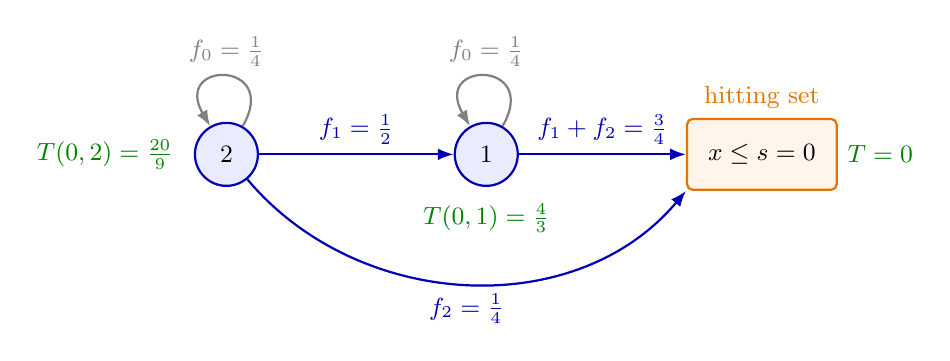
\begin{tikzpicture}[font=\small, >={Latex[length=2mm]},
  state/.style={circle, draw=blue!70!black, fill=blue!8, thick, minimum size=8mm}]
  \node[state] (s2) at (0,0) {$2$};
  \node[state] (s1) at (3.3,0) {$1$};
  \node[draw=orange!90!black, fill=orange!8, thick, rounded corners=2pt, minimum width=1.9cm,
        minimum height=0.9cm, align=center] (B) at (6.8,0) {$x\leq s=0$};
  \node[orange!90!black, anchor=south] at (B.north) {hitting set};
  % transitions
  \draw[->, blue!70!black, thick] (s2) -- node[above] {$f_1=\frac{1}{2}$} (s1);
  \draw[->, blue!70!black, thick] (s1) -- node[above] {$f_1+f_2=\frac{3}{4}$} (B);
  \draw[->, blue!70!black, thick] (s2) to[out=-50, in=-130] node[below] {$f_2=\frac{1}{4}$} (B.south west);
  % self-loops: no demand
  \draw[->, gray, thick] (s2) to[out=60, in=120, looseness=6] node[above] {$f_0=\frac{1}{4}$} (s2);
  \draw[->, gray, thick] (s1) to[out=60, in=120, looseness=6] node[above] {$f_0=\frac{1}{4}$} (s1);
  % values
  \node[green!50!black, anchor=east] at (-0.55,0) {$T(0,2)=\frac{20}{9}$};
  \node[green!50!black, anchor=north] at (3.3,-0.5) {$T(0,1)=\frac{4}{3}$};
  \node[green!50!black, anchor=west] at (B.east) {$T=0$};
\end{tikzpicture}
\end{document}
